\documentclass[man]{apa6}
\usepackage{lmodern}
\usepackage{amssymb,amsmath}
\usepackage{ifxetex,ifluatex}
\usepackage{fixltx2e} % provides \textsubscript
\ifnum 0\ifxetex 1\fi\ifluatex 1\fi=0 % if pdftex
  \usepackage[T1]{fontenc}
  \usepackage[utf8]{inputenc}
\else % if luatex or xelatex
  \ifxetex
    \usepackage{mathspec}
  \else
    \usepackage{fontspec}
  \fi
  \defaultfontfeatures{Ligatures=TeX,Scale=MatchLowercase}
\fi
% use upquote if available, for straight quotes in verbatim environments
\IfFileExists{upquote.sty}{\usepackage{upquote}}{}
% use microtype if available
\IfFileExists{microtype.sty}{%
\usepackage{microtype}
\UseMicrotypeSet[protrusion]{basicmath} % disable protrusion for tt fonts
}{}
\usepackage{hyperref}
\hypersetup{unicode=true,
            pdftitle={What measure of effect size when comparing two groups based on their means?},
            pdfauthor={Marie Delacre~\& Christophe Leys},
            pdfkeywords={keywords},
            pdfborder={0 0 0},
            breaklinks=true}
\urlstyle{same}  % don't use monospace font for urls
\usepackage{graphicx,grffile}
\makeatletter
\def\maxwidth{\ifdim\Gin@nat@width>\linewidth\linewidth\else\Gin@nat@width\fi}
\def\maxheight{\ifdim\Gin@nat@height>\textheight\textheight\else\Gin@nat@height\fi}
\makeatother
% Scale images if necessary, so that they will not overflow the page
% margins by default, and it is still possible to overwrite the defaults
% using explicit options in \includegraphics[width, height, ...]{}
\setkeys{Gin}{width=\maxwidth,height=\maxheight,keepaspectratio}
\IfFileExists{parskip.sty}{%
\usepackage{parskip}
}{% else
\setlength{\parindent}{0pt}
\setlength{\parskip}{6pt plus 2pt minus 1pt}
}
\setlength{\emergencystretch}{3em}  % prevent overfull lines
\providecommand{\tightlist}{%
  \setlength{\itemsep}{0pt}\setlength{\parskip}{0pt}}
\setcounter{secnumdepth}{0}
% Redefines (sub)paragraphs to behave more like sections
\ifx\paragraph\undefined\else
\let\oldparagraph\paragraph
\renewcommand{\paragraph}[1]{\oldparagraph{#1}\mbox{}}
\fi
\ifx\subparagraph\undefined\else
\let\oldsubparagraph\subparagraph
\renewcommand{\subparagraph}[1]{\oldsubparagraph{#1}\mbox{}}
\fi

%%% Use protect on footnotes to avoid problems with footnotes in titles
\let\rmarkdownfootnote\footnote%
\def\footnote{\protect\rmarkdownfootnote}


  \title{What measure of effect size when comparing two groups based on their means?}
    \author{Marie Delacre\textsuperscript{1}~\& Christophe Leys\textsuperscript{1}}
    \date{}
  
\shorttitle{Effect size}
\affiliation{
\vspace{0.5cm}
\textsuperscript{1} Université Libre de Bruxelles, Service of Analysis of the Data (SAD), Bruxelles, Belgium}
\keywords{keywords\newline\indent Word count: X}
\usepackage{csquotes}
\usepackage{upgreek}
\captionsetup{font=singlespacing,justification=justified}

\usepackage{longtable}
\usepackage{lscape}
\usepackage{multirow}
\usepackage{tabularx}
\usepackage[flushleft]{threeparttable}
\usepackage{threeparttablex}

\newenvironment{lltable}{\begin{landscape}\begin{center}\begin{ThreePartTable}}{\end{ThreePartTable}\end{center}\end{landscape}}

\makeatletter
\newcommand\LastLTentrywidth{1em}
\newlength\longtablewidth
\setlength{\longtablewidth}{1in}
\newcommand{\getlongtablewidth}{\begingroup \ifcsname LT@\roman{LT@tables}\endcsname \global\longtablewidth=0pt \renewcommand{\LT@entry}[2]{\global\advance\longtablewidth by ##2\relax\gdef\LastLTentrywidth{##2}}\@nameuse{LT@\roman{LT@tables}} \fi \endgroup}


\DeclareDelayedFloatFlavor{ThreePartTable}{table}
\DeclareDelayedFloatFlavor{lltable}{table}
\DeclareDelayedFloatFlavor*{longtable}{table}
\makeatletter
\renewcommand{\efloat@iwrite}[1]{\immediate\expandafter\protected@write\csname efloat@post#1\endcsname{}}
\makeatother
\usepackage{lineno}

\linenumbers

\authornote{

Correspondence concerning this article should be addressed to Marie Delacre, CP191, avenue F.D. Roosevelt 50, 1050 Bruxelles. E-mail: \href{mailto:marie.delacre@ulb.ac.be}{\nolinkurl{marie.delacre@ulb.ac.be}}}

\abstract{

}

\begin{document}
\maketitle

\hypertarget{intro}{%
\section{Intro}\label{intro}}

During decades, researchers in social science (Henson \& Smith, 2000) and education (Fan, 2001) have overestimated the ability of the null hypothesis (H0) testing to determine the importance of their results. The standard for researchers in social science is to define H0 as the absence of effect (Meehl, 1990). For example, when comparing the mean of two groups, researchers commonly test the H0 that there is no mean differences between groups (Steyn, 2000). Any effect that is significantly different from zero will be seen as sole support for a theory.

Such an approach has faced many criticisms among which the most relevant to our concern is that the null hypothesis testing highly depends on sample size: for a given alpha level and a given difference between groups, the larger the sample size, the higher the probability of rejecting the null hypothesis (Fan, 2001; Kirk, 2009; Olejnik \& Algina, 2000; Sullivan \& Feinn, 2012). It implies that even tiny differences could be detected as statistically significant with very large sample sizes (McBride, Loftis, \& Adkins, 1993)\footnote{Tiny differences might be due to sampling error, or to other factors than the one of interest: even under the assumption of random assignent (which is a necessary but not sufficient condition), it is almost impossible to be sure that the only difference between two conditions is the one defined by the factor of interest. Other tiny factors of no theoretical interest might slighly influence results, making the probability of getting an actual zero effect very low. This is what Meehl (1990) calls 'systematic noise'}.

Facing this argument, it has become an adviced practice to report the \emph{p}-value assorted by a measure of the effect size, that is, a quantitative measure of the magnitude of the experimental effect (Cohen, 1965; Fan, 2001; Hays, 1963). This practice is also highly endorsed by the American Psychological Association (APA) and the American Educational Research Association (AERA) (American Educational Research Association, 2006; American Psychological Association, 2010). However, limited studies properly report effect size in the last several decades.

First, there is a high confusion between the effect size and other related concepts such as the clininal significance {[}SEE NOTE LATER{]} of a result (i.e.~the relevance of an effect in real life). Moreover, there are several situations that call for effect size measures and in the current litterature, it's not always easy to know which measure using in a specific context.

Second, when used for inference, the main measures of effect sizes (i.e.~Cohen's \emph{d} and point-biserial \emph{r}) are submitted to a range of assumptions (i.e.~normality and heteroscedasticity) and these assumptions are known to be unrealistic in many research designs (Cain, Zhang, \& Yuan, 2017; Erceg-Hurn \& Mirosevich, 2008; Glass, Peckham, \& Sanders, 1972; Grissom, 2000; Micceri, 1989; Yuan, Bentler, \& Chan, 2004). As consequences many estimations of effect size are inaccurate and alter the robustness of the statistical conclusions. In the context of comparing two groups based on their means, Cohen's \(d_{s}\) is the dominant effect size measure used by researchers (Peng, Chen, Chiang, \& Chiang, 2013; Shieh, 2013). We will argue that, like Student's \emph{t}-test, this measure rely on the often untenable assumptions of normality and homogeneity of variances (Cumming, 2013; Grissom \& Kim, 2005; Kelley, 2005; Shieh, 2013). While it is becoming more common in statistical software to present Welch's \emph{t}-test by default, when performing a \emph{t}-test (i.e., R, Minitab), similar issues for the measures of effect sizes has received less attention (Shieh, 2013) and Cohen's \(d_{s}\) remains persistent \footnote{For example, in Jamovi, Cohen's ds is provided, whatever one performs Student's or Welch's t-test}.

In sum the aim of this paper is threefold:\\
1. Clearly define what is (and what is not) a measure of effect size;\\
2. Listing the different situations that call for effect sizes measure and reviewing which measure is appropriate in which circumstance;\\
3. Define different properties of a good effect size estimator and discuss the impact of assumptions violations on the robustness of the measures of effect size, based on simulations.

\hypertarget{measure-of-effect-size-what-it-is-what-it-is-not}{%
\section{Measure of effect size: what it is, what it is not}\label{measure-of-effect-size-what-it-is-what-it-is-not}}

The effect size is commonly refered to the practical significance of a test. Grissom and Kim (2005) define the effect size as the extent to which results differ from what is implied by the null hypothesis. In the context of the comparison of two groups based on their mean, depending on the defined null hypothesis (considering the absence of effect as the null hypothesis), we could define the effect size either as the magnitude of differences between parameters of two populations groups are extracted from (e.g.~the mean; Peng \& Chen, 2014) or as the magnitude of the relation between one dichotomous factor and one dependent variable (American Educational Research Association, 2006). Both definitions refers to as the most famous families of measures of effect sizes {[}Rosenthal\_1994{]}: respectively the \emph{d}-family and the \emph{r}-family.

Very often, the contribution of the measures of effect size is overestimated.

First, benchmarks about what should be a small, medium or large effect size might have contribued at seeing the effect size as a measure of the importance or the relevance of an effect in real life, but it is not (Stout \& Ruble, 1995). The effect size is only a mathematical indicator of the magnitude of a difference, which depends on the way a variable is converted into numerical indicator. In order to assess the meaningfulness of an effect, we should be able to relate this effect with behaviors/meaningful consequences in the real world (Andersen, McCullagh, \& Wilson, 2007). For example, let us imagine a sample of students in serious school failure who are randomly divided into two groups: an experimental group following a training program and a control group. At the end of the training, students in the experimental group have on average significantly higher scores on a test than students in the control group, and the difference is large (e.g.~30 percents). Does it mean that students in the experimental condition will be able to pass to the next grade and to continue normal schooling? Whether the computed magnitude of difference is an important, meaningful change in everyday life refers to another construct: the \emph{clinical significance} (Bothe \& Richardson, 2011). {[}I DON'T LIKE THE WORD \enquote{CLINICAL} BECAUSE IT'S NOT GENERAL ENOUGH.A MEANINGFUL SIGNIFICANCE COULD BE SOCIAL, PERSONAL, CLINICAL, PROFESIONNAL\ldots{} ANY IDEA OF A MORE GENERAL WORD?{]}. It refers to the interpretation of treatment outcomes and is neither statistical nor mathematical, it is related to underlying theory that posits an empirical hypothesis. In other words, the relation between \emph{practical} and \emph{clinical} significance is more a theoretical argument than a statistical one.

Second, in the context of the comparison of two groups based on their means, it should not replace the null hypothesis testing. Statistical testing allows the researcher to determine whether the oberved departure from H0 occured by chance or not (Stout \& Ruble, 1995) while effect size estimators allow to assess the practical signficance of an effect, and as reminds Fan (2001) \enquote{a practically meaningful outcome may also have occured by chance, and consequently, is not trustworthy}. For this reason, the use of confidence intervals around the effect size estimate is highly recommended (Bothe \& Richardson, 2011).

\hypertarget{different-goals-of-measures-of-effect-sizes}{%
\section{Different goals of measures of effect sizes}\label{different-goals-of-measures-of-effect-sizes}}

Effect size measures can be used for \emph{inferential} purposes:\\
- The effect sizes from previous studies can be used in a priori power analysis when planning a new study (Lakens, 2013; Prentice \& Miller, 1990; Stout \& Ruble, 1995; Sullivan \& Feinn, 2012; Wilkinson \& the Task Force on Statistical Inference, 1999)\\
- To compute confidence intervals (Shieh, 2013)

Measures of effect size can also be used for \emph{comparative} purposes, i.e.~to assess the stability of results across designs, analysis, samples sizes (Wilkinson \& the Task Force on Statistical Inference, 1999). It includes:\\
- To compare results of 2 or more studies (Prentice \& Miller, 1990)\\
- To incorporate results in meta-analysis (Lakens, 2013; Li, 2016; Nakagawa \& Cuthill, 2007; Stout \& Ruble, 1995; Wilkinson \& the Task Force on Statistical Inference, 1999)

Finally, effect size measures can be used for \emph{interpretive} purposes: in order to assess the practical significance of a result (beyond statistical significance; Lakens, 2013; American Psychological Association, 2010; Prentice \& Miller, 1990)

When used for \emph{inference}, effect size measures should meet some mathematical properties (see next section). According to the statistical properties of Welch's statistic, in the context of heteroscedasticity, it does not seem possible to define a proper measure of effect size without taking the specificity of the design (and more specifically the sample size allocation ratio) into account in the calculation of the group variance (Shieh, 2013). On the other side, generality is required for comparative and interpretive purposes (Cumming, 2013).

\hypertarget{robust-measures}{%
\section{Robust measures}\label{robust-measures}}

\hypertarget{properties-of-a-good-effect-size-estimator-for-inferential-purposes}{%
\subsection{Properties of a good effect size estimator (for inferential purposes)}\label{properties-of-a-good-effect-size-estimator-for-inferential-purposes}}

The value of the estimate of an estimator depends on the sampling. That is to say, based on different samples extracted from the same population, one would obtain different estimates of the same estimator. The \emph{sampling distribution} of the estimator is the distribution of all estimates, based on all possible samples of size \emph{n} extracted from one population. Studying the sampling distribution is very useful, as it allows to assess the goodness of an effect size estimator and more specifically, three desirable properties of a good estimator: \textbf{unbiasedness}, \textbf{consistency} and \textbf{efficiency}.

An estimator is unbiased if the distribution of estimates is centered around the true population parameter. On the other hand, an estimator is positively (or negatively) biased if the distribution is centered around a value that is higher (or smaller) than the true populatione parameter (see Figure 1). In other words, the bias tells us if estimates are good, on average. The \emph{bias} of a point estimator \(\hat{\delta}\) can be computed as follows:

\begin{equation} 
\hat{\delta}_{bias}=E(\hat{\delta})-\delta
\label{eq:BIAS}
\end{equation}

Where \(E(\hat{\delta})\) is the mean of the sampling distribution of the estimator and \(\delta\) is the true parameter.

In order to compare the \emph{bias} of a point estimator for different true population parameters, we can compute the bias divided by \(\delta\).

\begin{equation} 
\hat{\delta}_{bias}=\frac{E(\hat{\delta})-\delta}{\delta}
\label{eq:BIASRATE}
\end{equation}

\begin{figure}
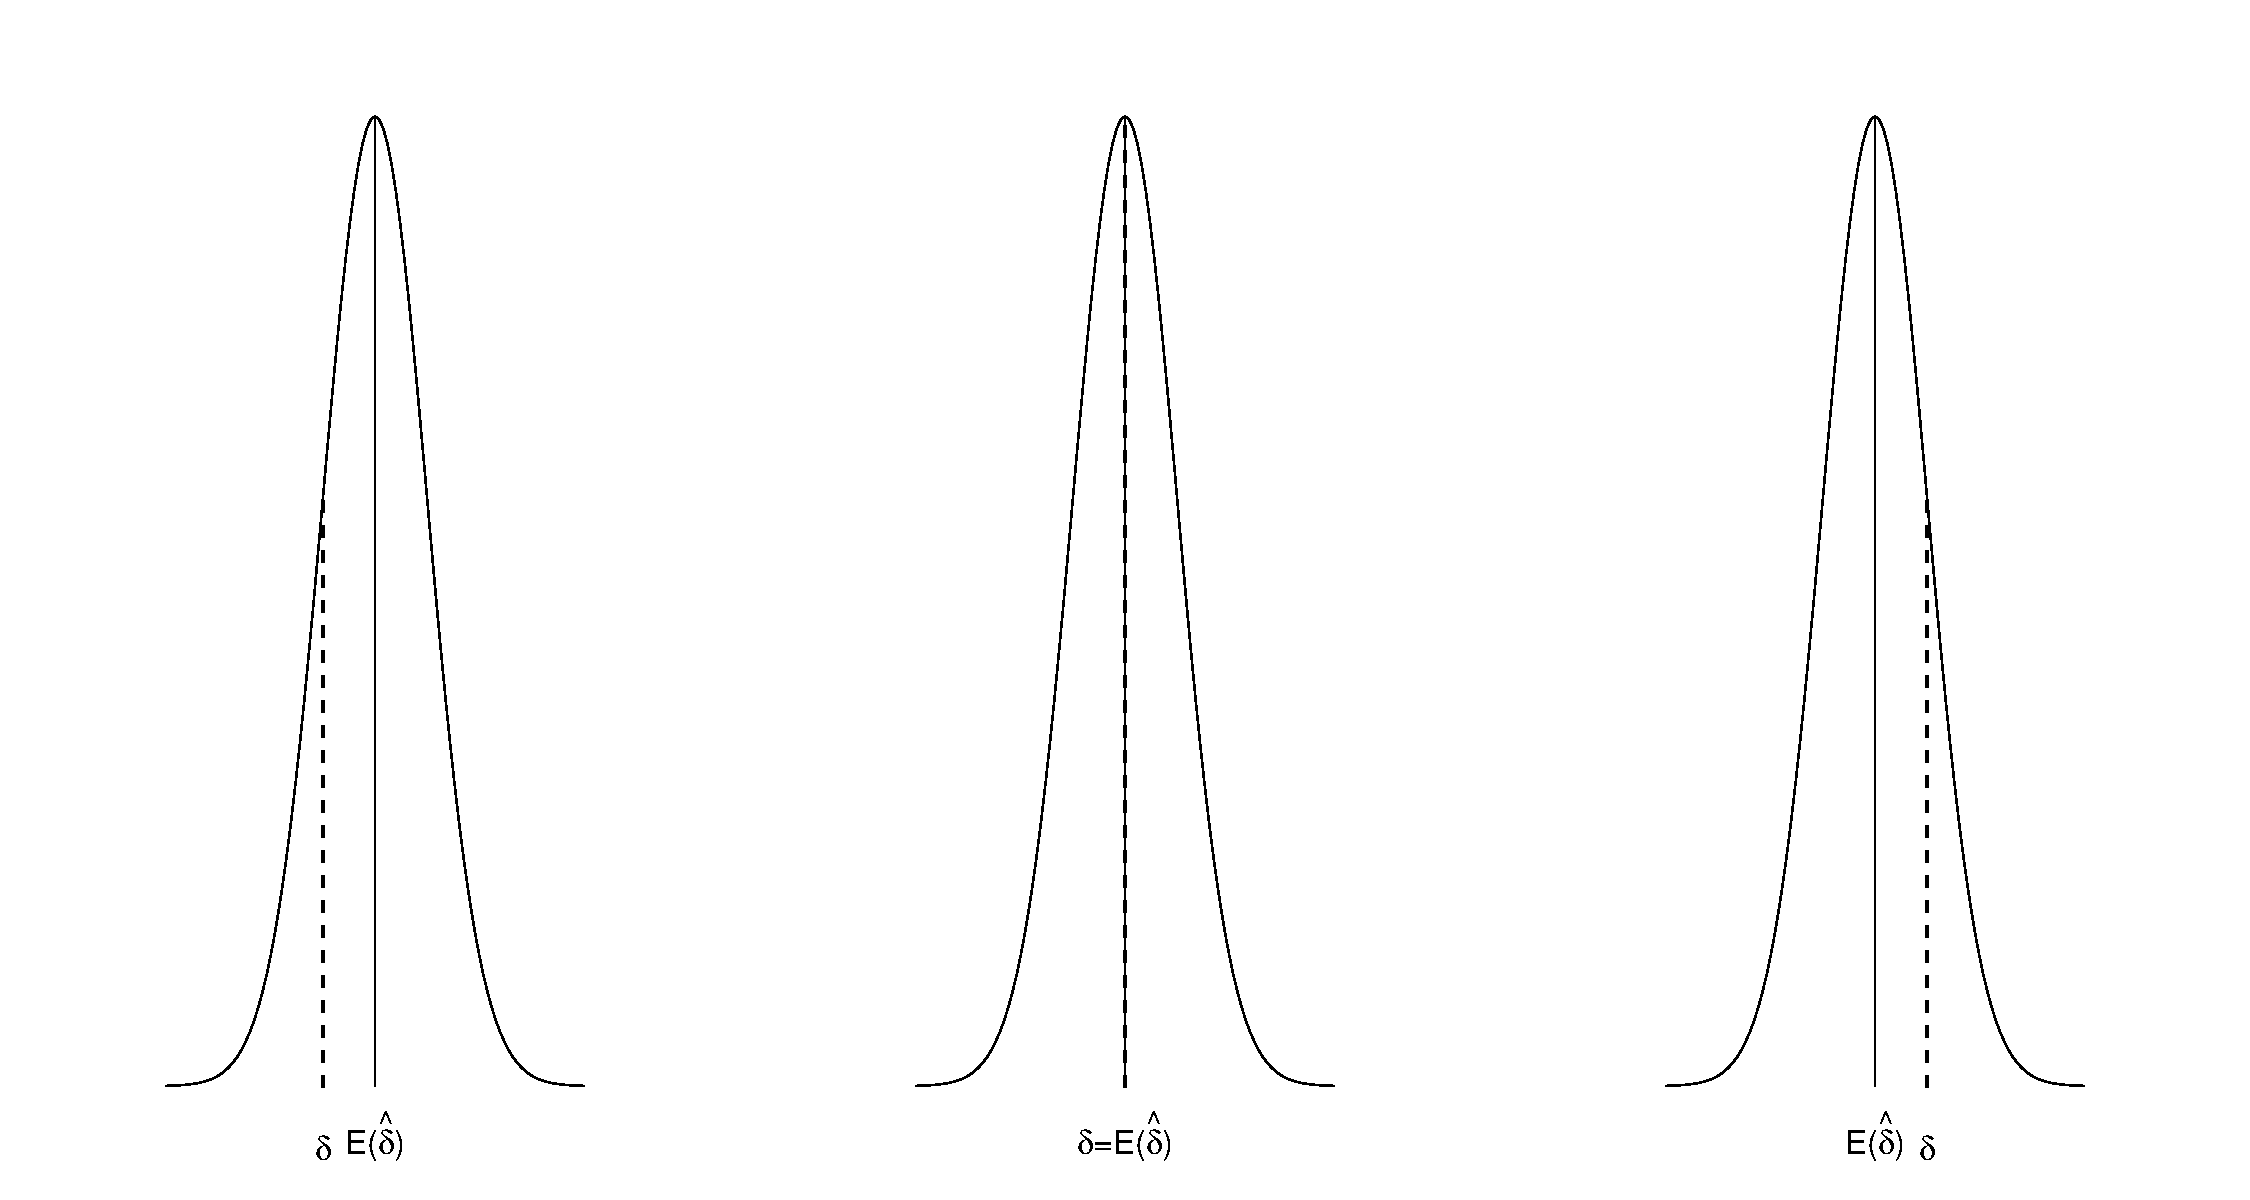
\includegraphics[width=400px]{ES_files/figure-latex/unnamed-chunk-1-1} \caption{Samplig distribution for a positively biased (left), an unbiased (center) and a negatively biased estimator (right)}\label{fig:unnamed-chunk-1}
\end{figure}

Bias informs us about the goodness of estimates averages, but says nothing about individual estimates. Imagine a situation where the distribution of estimates is centered around the real parameter but with such a large variance that some point estimates are very far from the center. It would be problematic, as long as we have only one estimate, the one based on our sample, and we don't know how far is this estimate from the center of the sampling distribution. We hope that \emph{all} possible estimates are close enough of the true population parameter, in order to be sure that for \emph{any} estimate, one has a correct estimation of the real parameter. In other words, we expect the variability of estimates around the true population parameter to be as small as possible. It refers to the \textbf{efficiency} of the point estimator (\(\hat{\delta}\)) and can be computed as follows:

\begin{equation} 
\hat{\delta}_{efficiency}=Var(\hat{\delta})
\label{eq:EFFICIENCY}
\end{equation}

Among all unbiased estimators, the more efficient will be the one with the smallest variance.

Note that both unbiasedness and efficiency are very important. Remember that we hope that \emph{any} possible estimate is close of the real parameter. An unbiased estimator with such a large variance that somes estimates are extremely far from the real parameter is as undesirable as a parameter which is highly biased. In some situations, it is better to have a very slightly biased estimator with a tigh shape around the biased value, so each estimate \enquote{misses} the real parameter a little, than a biased estimator with a large variance {[}Ref to add: \url{https://eranraviv.com/bias-vs-consistency/}{]}. Because both \emph{unbiasedness} and \emph{efficiency} must be considered, it is interesting to compute an indicator that take simultaneously both properties into account (Wackerly, Mendenhall, \& Scheaffer, 2008). The \emph{mean square error} of a point estimator \(\hat{\delta}\) is defined as follows:

\begin{equation} 
MSE(\hat{\delta})=E[(\hat{\delta}-\delta)^2]
\label{eq:MSE1}
\end{equation}

It can be proven that the \emph{mean square error} is a function of the bias and the variance of \(\hat{\delta}\) :

\begin{equation} 
MSE(\hat{\delta})=\hat{\delta}_{efficiency}+\hat{\delta}_{bias}^2
\label{eq:MSE2}
\end{equation}

Finally, the last property if a good point estimator is \textbf{consistency}: consistency means that the bigger the sample size, the closer the estimate of the population parameter. In other words, the estimates \emph{converge} to the true population parameter.

\hypertarget{properties-of-a-good-effect-size-estimator-for-comparative-and-interpretive-purposes}{%
\subsection{Properties of a good effect size estimator (for comparative and interpretive purposes)}\label{properties-of-a-good-effect-size-estimator-for-comparative-and-interpretive-purposes}}

\textbf{Interpretability}

\hypertarget{simulations}{%
\subsection*{Simulations}\label{simulations}}
\addcontentsline{toc}{subsection}{Simulations}

\hypertarget{refs}{}
\leavevmode\hypertarget{ref-AERA_2006}{}%
American Educational Research Association. (2006). Standards for reporting on empirical social science research in aera publications. \emph{Educational Researcher}, \emph{35}, 33--40. doi:\href{https://doi.org/10.3102/0013189X035006033}{10.3102/0013189X035006033}

\leavevmode\hypertarget{ref-APA_2010}{}%
American Psychological Association. (2010). \emph{Publication manual of the american psychological association {[}apa{]} (6 ed.)} (American Psychological Association.). Washington, DC:

\leavevmode\hypertarget{ref-Andersen_et_al_2007}{}%
Andersen, M. B., McCullagh, P., \& Wilson, G. J. (2007). But what do the numbers really tell us? Arbitrary metrics and effect size reporting in sport psychology research. \emph{Journal of Sport \& Exercise Psychology}, \emph{29}, 664--672.

\leavevmode\hypertarget{ref-Bothe_Richardson_2011}{}%
Bothe, A. K., \& Richardson, J. D. (2011). Statistical, practical, clinical, and personal significance: Definitions and applications in speech-language pathology. \emph{American Journal of Speech-Language Pathology}, \emph{20}, 233--242.

\leavevmode\hypertarget{ref-Cain_et_al_2017}{}%
Cain, M. K., Zhang, Z., \& Yuan, K.-H. (2017). Univariate and multivariate skewness and kurtosis for measuring nonnormality: Prevalence, influence and estimation. \emph{Behavior Research Methods}, \emph{49}(5), 1716--1735. doi:\href{https://doi.org/10.3758/s13428-016-0814-1}{10.3758/s13428-016-0814-1}

\leavevmode\hypertarget{ref-Cohen_1965}{}%
Cohen, J. (1965). Some statistical issues in psychological research. In \emph{Handbook of clinical psychology} (B. B. Wolman., pp. 95--121). New York: McGraw-Hill.

\leavevmode\hypertarget{ref-Cumming_2013}{}%
Cumming, G. (2013). Cohen's d needs to be readily interpretable: Comment on shieh (2013). \emph{Behavior Research Methods}, \emph{45}, 968--971. doi:\href{https://doi.org/10.3758/s13428-013-0392-4}{10.3758/s13428-013-0392-4}

\leavevmode\hypertarget{ref-Erceg-Hurn_Mirosevich_2008}{}%
Erceg-Hurn, D. M., \& Mirosevich, V. M. (2008). Modern robust statistical methods: An easy way to maximize the accuracy and power of your research. \emph{American Psychologist}, \emph{63}(7), 591--601. doi:\href{https://doi.org/10.1037/0003-066X.63.7.591}{10.1037/0003-066X.63.7.591}

\leavevmode\hypertarget{ref-Fan_2001}{}%
Fan, X. (2001). Statistical significance and effect size in education research: Two sides of a coin. \emph{Journal of Educational Research}, \emph{94}(5), 275--282. doi:\href{https://doi.org/10.1080/00220670109598763}{10.1080/00220670109598763}

\leavevmode\hypertarget{ref-Glass_et_al_1972}{}%
Glass, G. V., Peckham, P. D., \& Sanders, J. R. (1972). Consequences of failure to meet assumptions underlying the fixed effects analyses of variance and covariance. \emph{Review of Educational Research}, \emph{42}(3), 237--288. doi:\href{https://doi.org/10.3102/00346543042003237}{10.3102/00346543042003237}

\leavevmode\hypertarget{ref-Grissom_2000}{}%
Grissom, R. J. (2000). Heterogeneity of variance in clinical data. \emph{Journal of Consulting and Clinical Psychology}, \emph{68}(1), 155--165. doi:\href{https://doi.org/10.1037//0022-006x.68.1.155}{10.1037//0022-006x.68.1.155}

\leavevmode\hypertarget{ref-Grissom_and_kim_2005}{}%
Grissom, R. R., \& Kim, J. J. (2005). \emph{Effect size for research: A broad practical approach.} (Lawrence Erlbaum Associates, Mahwah, N.J.). London.

\leavevmode\hypertarget{ref-Hays_1963}{}%
Hays, W. L. (1963). \emph{Statistics for psychologists} (Holt, Rinehart \& Winston.). New York.

\leavevmode\hypertarget{ref-Henson_Smith_2000}{}%
Henson, R. I., \& Smith, A. D. (2000). State of the art in statistical significance and effect size reporting: A review of the APA task force report and current trends. \emph{Journal of Research and Development in Education}, \emph{33}(4), 285--296.

\leavevmode\hypertarget{ref-Kelley_2005}{}%
Kelley, K. (2005). The effects of nonnormal distributions on confidence intervales around the standardized mean difference: Bootstrap and parametric confidence intervals. \emph{Educational and Psychological Measurement}, \emph{65}(1), 51--69. doi:\href{https://doi.org/10.1177/0013164404264850}{10.1177/0013164404264850}

\leavevmode\hypertarget{ref-Kirk_2009}{}%
Kirk, R. E. (2009). Practical significance: A concept whose time has come. \emph{Educational and Psychological Measurement}, \emph{56}(5), 746--759. doi:\href{https://doi.org/10.1177/0013164496056005002\%20}{10.1177/0013164496056005002 }

\leavevmode\hypertarget{ref-Lakens_2013}{}%
Lakens, D. (2013). Calculating and reporting effect sizes to facilitate cumulative science: A practical primer for t-tests and ANOVAs. \emph{Frontiers in Psychology}, \emph{4}(863), 1--12. doi:\href{https://doi.org/10.3389/fpsyg.2013.00863}{10.3389/fpsyg.2013.00863}

\leavevmode\hypertarget{ref-Li_2016}{}%
Li, J. (2016). Effect size measures in a two-independent-samples case with nonnormal and nonhomogeneous data. \emph{Behavior Research Methods}, \emph{48}(4), 1560--1574. doi:\href{https://doi.org/10.3758/s13428-015-0667-z}{10.3758/s13428-015-0667-z}

\leavevmode\hypertarget{ref-McBride_et_al_1993}{}%
McBride, G. B., Loftis, J. C., \& Adkins, N. C. (1993). What do significance tests really tell us about the environment? \emph{Environmental Management}, \emph{17}(4), 423--432.

\leavevmode\hypertarget{ref-Meehl_1990}{}%
Meehl, P. E. (1990). Appraising and amending theories: The strategy of Lakatosian defense and two principles that warrant it. \emph{Psychological Inquiry}, \emph{1}(2), 108--141.

\leavevmode\hypertarget{ref-Micceri_1989}{}%
Micceri, T. (1989). The unicorn, the normal curve, and other improbable creatures. \emph{Psychological Bulletin}, \emph{105}(1), 156--166. doi:\href{https://doi.org/10.1037/0033-2909.105.1.156}{10.1037/0033-2909.105.1.156}

\leavevmode\hypertarget{ref-Nakagawa_and_Cuthill_2007}{}%
Nakagawa, S., \& Cuthill, I. C. (2007). Effect size, confidence interval and statistical significance: A practical guide for biologists. \emph{Biological Reviews}, \emph{82}, 591--605. doi:\href{https://doi.org/10.1111/j.1469-185X.2007.00027.x}{10.1111/j.1469-185X.2007.00027.x}

\leavevmode\hypertarget{ref-Olejnik_Algina_2000}{}%
Olejnik, S., \& Algina, J. (2000). Measures of effect size for comparative studies: Applications, interpretations, and limitations. \emph{Contemporary Educational Psychology}, \emph{25}, 241--286. doi:\href{https://doi.org/10.1006/ceps.2000.1040}{10.1006/ceps.2000.1040}

\leavevmode\hypertarget{ref-Peng_and_Chen_2014}{}%
Peng, C.-Y., \& Chen, L.-T. (2014). Beyond cohen's d: Alternative effect size measures for between-subject designs. \emph{THE JOURNAL OF EXPERIMENTAL EDUCATION}, \emph{82}(1), 22--50. doi:\href{https://doi.org/10.1080/00220973.2012.745471}{10.1080/00220973.2012.745471}

\leavevmode\hypertarget{ref-Peng_et_al_2013}{}%
Peng, C.-Y., Chen, L.-T., Chiang, H.-M., \& Chiang, Y.-C. (2013). The Impact of APA and AERA Guidelines on Effect size Reporting. \emph{Contemporary Educational Psychology}, \emph{82}(1), 22--50. doi:\href{https://doi.org/10.1080/00220973.2012.745471}{10.1080/00220973.2012.745471}

\leavevmode\hypertarget{ref-Prentice_Miller_1992}{}%
Prentice, D., \& Miller, D. T. (1990). When small effects are impressive. \emph{Psychological Bulletin}, \emph{112}(1), 160--164.

\leavevmode\hypertarget{ref-Shieh_2013}{}%
Shieh, G. (2013). Confidence intervals and sample size calculations for the weighted eta-squared effect sizes in one-way heteroscedastic ANOVA. \emph{Behavior Research Methods}, \emph{45}(1), 2--37. doi:\href{https://doi.org/10.3758/s13428-012-0228-7}{10.3758/s13428-012-0228-7}

\leavevmode\hypertarget{ref-Steyn_2000}{}%
Steyn, H. S. (2000). Practical significance of the difference in means. \emph{Journal of Industrial Psychology}, \emph{26}(3), 1--3.

\leavevmode\hypertarget{ref-Stout_Ruble_1995}{}%
Stout, D. D., \& Ruble, T. L. (1995). Assessing the practical signficance of empirical results in accounting education research: The use of effect size information. \emph{Journal of Accounting Education}, \emph{13}(3), 281--298.

\leavevmode\hypertarget{ref-Sullivan_Feinn_2012}{}%
Sullivan, G., \& Feinn, R. (2012). Using effect size---or why the p value is not enough. \emph{Journal of Graduate Medical Education}, 279--282. doi:\href{https://doi.org/10.4300/JGME-D-12-00156.1}{10.4300/JGME-D-12-00156.1}

\leavevmode\hypertarget{ref-Wackerly_et_al_2008}{}%
Wackerly, D. D., Mendenhall, W., \& Scheaffer, R. L. (2008). \emph{Mathematical statistics with applications (7th edition)} (Brooks/Cole, Cengage Learning.). Belmont, USA.

\leavevmode\hypertarget{ref-Wilkinson_1999}{}%
Wilkinson, L., \& the Task Force on Statistical Inference. (1999). Statistical methods in psychology journals: Guidelines and explanations. \emph{American Psychologist}, \emph{54}(8), 594--604.

\leavevmode\hypertarget{ref-Yuan_et_al_2004}{}%
Yuan, K.-H., Bentler, P. M., \& Chan, W. (2004). Structural equation modeling with heavy tailed distributions. \emph{Psychometrika}, \emph{69}(3), 421--436. doi:\href{https://doi.org/10.1007/bf02295644}{10.1007/bf02295644}


\end{document}
